\section{Experimental Results}
\label{sec:results}

We report macro-averaged per-page metrics across all successfully processed test images: Character Error Rate (\textbf{CER} $\downarrow$), Word Error Rate (\textbf{WER} $\downarrow$), order-insensitive bag-of-words token \textbf{Precision}, \textbf{Recall}, and \textbf{F1} ($\uparrow$), and average \textbf{Inference Time} (seconds/image $\downarrow$).

\subsection{Quantitative Results}
Table~\ref{tab:overall_results} presents overall results on the 3,000-page OPRB test subset. \textbf{RapidOCR (PP-OCRv6)} attains best overall accuracy, achieving lowest CER ($0.3317$), lowest WER ($0.4283$), and highest token F1 ($0.7678$). \textbf{PaddleOCR-VL} ranks second overall (CER $0.4194$, WER $0.5886$, F1 $0.6765$), outperforming \textbf{Tesseract v5.5} (CER $0.4768$, F1 $0.5194$) and \textbf{EasyOCR} (CER $0.5930$, F1 $0.3556$). While \textbf{Florence-2-base} achieves fast inference ($0.82$\,s/img on dual T4 GPUs), its accuracy degrades severely (CER $1.0415$, Recall $0.2730$) due to an architectural bottleneck: its generation output is strictly capped at $1024$ tokens (\texttt{max\_new\_tokens=1024}). Because OPRB pages average $622.5$ words (often exceeding $1,000$--$1,500$ subword tokens), generation truncates mid-page; ungenerated tokens are penalized as deletions, mechanically driving CER $>1.0$ and deflating Recall.

\begin{table}[H]
    \centering
    \caption{Overall macro-averaged performance on the OPRB test evaluation subset (3,000 images).}
    \label{tab:overall_results}
    \footnotesize
    \renewcommand{\arraystretch}{0.85}
    \begin{tabular}{lccccccc}
        \toprule
        \textbf{Model} & \textbf{Category} & \textbf{CER $\downarrow$} & \textbf{WER $\downarrow$} & \textbf{Precision $\uparrow$} & \textbf{Recall $\uparrow$} & \textbf{F1 $\uparrow$} & \textbf{Time (s/img) $\downarrow$} \\
        \midrule
        Florence-2-base & VLM & 1.0415 & 0.8008 & 0.5559 & 0.2730 & 0.3519 & \textbf{0.82} \\
        PaddleOCR-VL & VLM & 0.4194 & 0.5886 & 0.7721 & 0.6471 & 0.6765 & 9.13 \\
        RapidOCR (PP-OCRv6) & OCR & \textbf{0.3317} & \textbf{0.4283} & \textbf{0.8691} & \textbf{0.7072} & \textbf{0.7678} & 0.84 \\
        Tesseract v5.5 & OCR & 0.4768 & 0.6451 & 0.6431 & 0.4556 & 0.5194 & 0.95 \\
        EasyOCR 1.7.2 & OCR & 0.5930 & 0.8232 & 0.4426 & 0.3066 & 0.3556 & 2.57 \\
        \bottomrule
    \end{tabular}
\end{table}

\subsection{Text vs.\ Non-Text Region Occlusions}
Table~\ref{tab:region_comparison} compares model performance on \texttt{text} (2,000 pages) versus \texttt{nontext} (1,000 pages) occlusions. Models exhibit distinct degradation patterns: RapidOCR achieves higher token F1 on text occlusions ($0.7854$) than on non-text occlusions ($0.7326$), though non-text corruptions produce higher CER ($0.4646$ vs $0.2652$) due to non-text background artifacts being falsely detected as text tokens. PaddleOCR-VL ($0.7013$ vs.\ $0.6268$ F1), Tesseract, and EasyOCR degrade similarly, while Florence-2 remains constrained by generation truncation across both subsets.

\begin{table}[H]
    \centering
    \caption{Performance comparison by occlusion region (\texttt{text} vs.\ \texttt{nontext}).}
    \label{tab:region_comparison}
    \footnotesize
    \renewcommand{\arraystretch}{0.85}
    \begin{tabular}{lcccc}
        \toprule
        & \multicolumn{2}{c}{\textbf{\texttt{text} (2,000)}} & \multicolumn{2}{c}{\textbf{\texttt{nontext} (1,000)}} \\
        \cmidrule(lr){2-3} \cmidrule(lr){4-5}
        \textbf{Model} & \textbf{CER $\downarrow$} & \textbf{F1 $\uparrow$} & \textbf{CER $\downarrow$} & \textbf{F1 $\uparrow$} \\
        \midrule
        Florence-2-base & 1.0265 & 0.3640 & 1.0714 & 0.3277 \\
        PaddleOCR-VL & 0.3562 & 0.7013 & 0.5457 & 0.6268 \\
        RapidOCR (PP-OCRv6) & \textbf{0.2652} & \textbf{0.7854} & \textbf{0.4646} & \textbf{0.7326} \\
        Tesseract v5.5 & 0.4183 & 0.5393 & 0.5939 & 0.4796 \\
        EasyOCR 1.7.2 & 0.5619 & 0.3718 & 0.6553 & 0.3232 \\
        \bottomrule
    \end{tabular}
\end{table}

\subsection{Robustness Analysis}
We group recognition errors by occlusion type and density across evaluated models. Across all corruptions, \textbf{RapidOCR} demonstrates the highest robustness (WER $0.4190$--$0.4583$), followed by \textbf{PaddleOCR-VL} ($0.5730$--$0.6644$), \textbf{Tesseract} ($0.6441$--$0.6780$), \textbf{Florence-2} ($0.7950$--$0.8071$), and \textbf{EasyOCR} ($0.8228$--$0.8271$). Natural simulations (\texttt{Sim}) yield lower WER ($0.4190$ on RapidOCR) than opaque streaks (\texttt{Black\_Ink}, $0.4362$) and scattered noise (\texttt{Through\_Dust}, $0.4583$), whereas PaddleOCR-VL performs slightly better on \texttt{Black\_Ink} ($0.5730$) than \texttt{Sim} ($0.6034$) and \texttt{Through\_Dust} ($0.6644$). Scaling occlusion density steadily degrades performance: on \texttt{Black\_Ink}, RapidOCR WER climbs from $0.4145$ ($0.5\%$) to $0.4288$ ($1.0\%$) and $0.4654$ ($2.0\%$), Tesseract WER increases from $0.6233$ to $0.6752$, and PaddleOCR-VL rises from $0.5583$ ($0.5\%$) to $0.6171$ ($2.0\%$).

\begin{figure}[H]
    \centering
    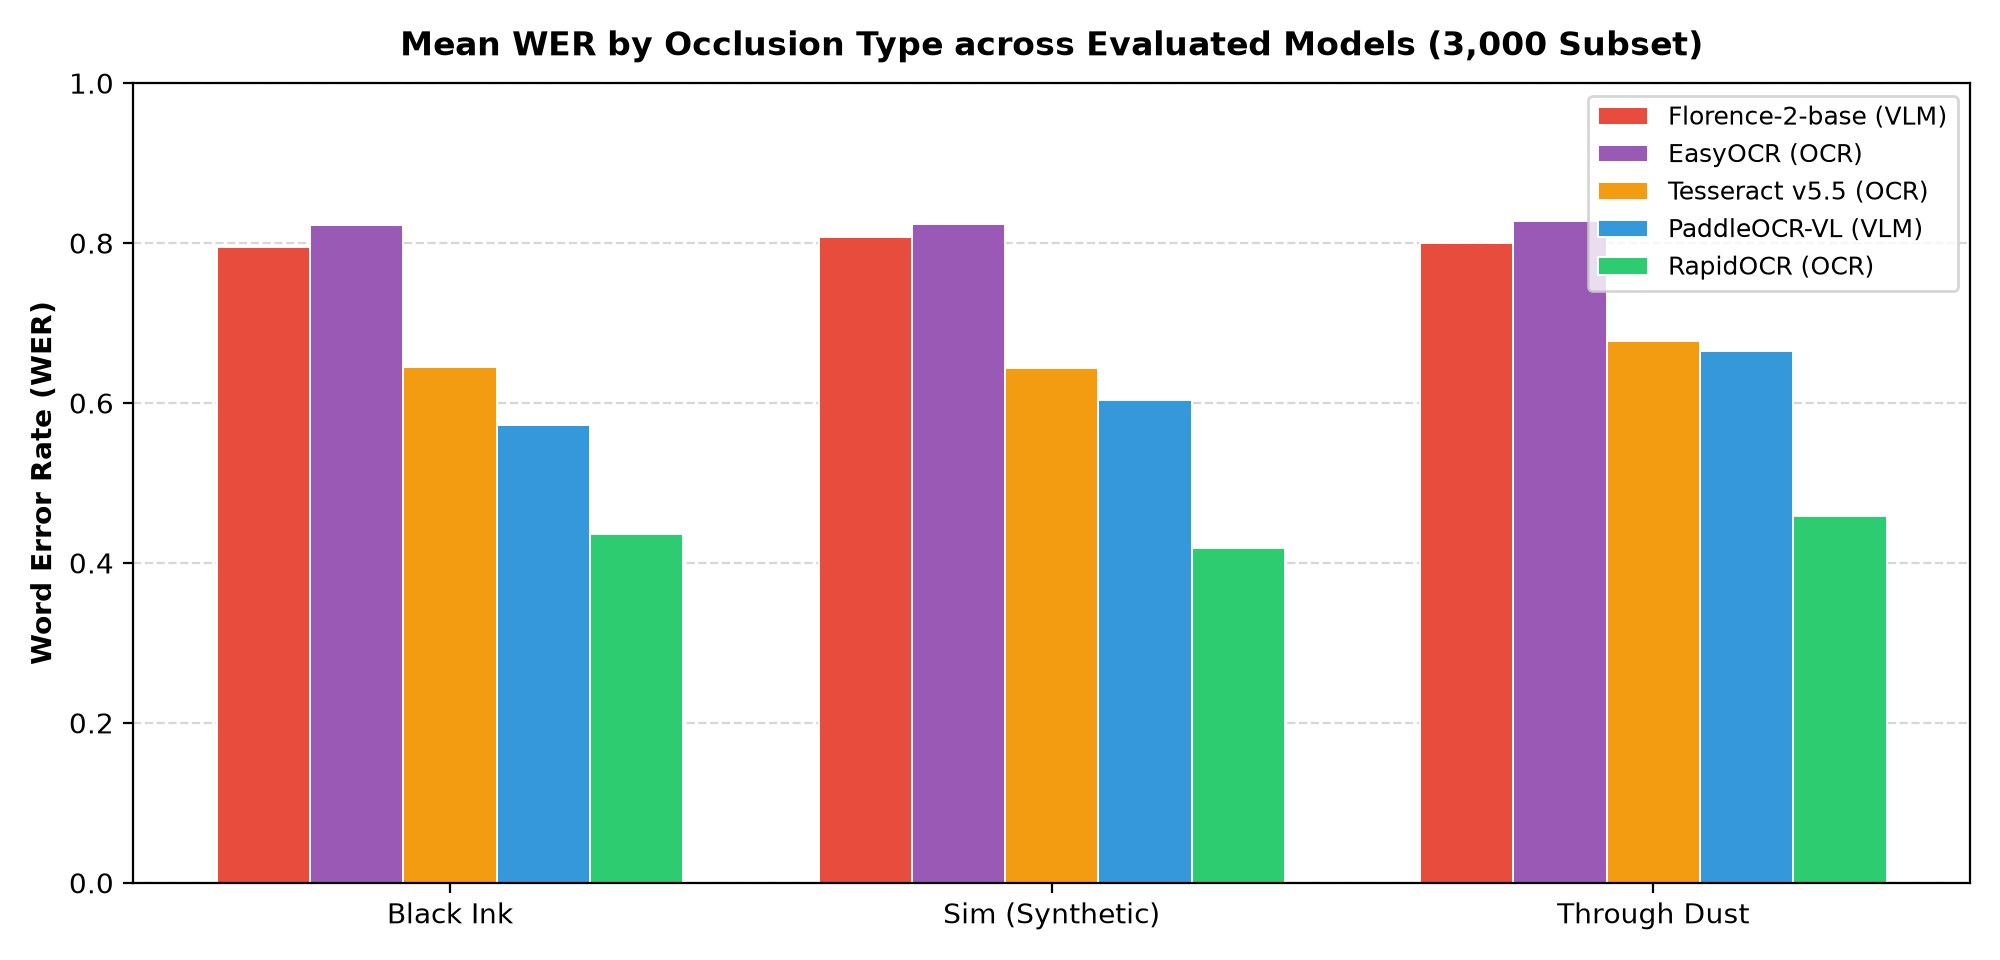
\includegraphics[width=0.75\columnwidth]{figures/wer_by_occlusion_type.png}
    \caption{Mean WER across occlusion types on OPRB test images.}
    \label{fig:occlusion_types}
\end{figure}

\subsection{Qualitative Examples}
We examine representative test predictions from \url{per_image_results.csv} illustrating key recognition behaviors under different corruptions:
\begin{itemize}[leftmargin=*,itemsep=2pt]
    \item \textbf{Successful Robustness (\texttt{spdy\_tr\_0}, \texttt{Black\_Ink}, 1.0\%):} RapidOCR transcribes dense academic text with near-perfect fidelity ($\text{CER}=0.0043$). Bounding box detection traces text lines across ink streaks without fragmentation: \\
    \hspace*{1em}\textbf{GT:} ``\textit{The Effect of Network and Infrastructural Variables on SPDY's Performance...}'' \\
    \hspace*{1em}\textbf{Pred:} ``\textit{The Effect of Network and Infrastructural Variables on SPDY's Performance...}''

    \item \textbf{Omission via Dense Masking (\texttt{paper\_7\_ori}, \texttt{Black\_Ink}, 2.0\%):} Heavy 2.0\% ink streaks obliterate entire text segments ($\text{CER}=0.6972$). The recognizer skips severed words and outputs fragmented characters, causing unavoidable token deletions.

    \item \textbf{Spurious Artifact Insertion (\texttt{paper\_19\_ori}, \texttt{Sim}, nontext):} Non-text chart axes and tick marks in figure regions are falsely detected as alphanumeric sequences ($\text{CER}=1.7050$), inserting hallucinated strings before the actual caption text.
\end{itemize}

\subsection{Efficiency Analysis}
Dedicated OCR pipelines demonstrate exceptional parameter efficiency: \textbf{RapidOCR} operates with only $\approx$15M parameters ($\approx$17\,MB) and processes full pages in $0.84$\,s on a local GPU while attaining best recognition accuracy ($\text{CER}=0.3317$, token $\text{F1}=0.7678$). \textbf{Tesseract v5.5} achieves competitive $0.95$\,s/image processing on a 16-thread CPU. In contrast, \textbf{EasyOCR} ($\approx$40M parameters) requires $2.57$\,s/image even with GPU batching (size 32) and obtains lower F1 ($0.3556$). Among generative VLMs, \textbf{Florence-2-base} ($\approx$232M parameters, $2\times$ Tesla T4) achieves $0.82$\,s/image but suffers from high character error rates ($\text{CER}=1.0415$) because its $1024$-token generation budget truncates lengthy documents. \textbf{PaddleOCR-VL} ($\approx$0.9B parameters, $2\times$ Tesla T4) mitigates truncation with a $2048$-token budget and anti-repetition decoding to reach second-best accuracy ($\text{F1}=0.6765$), but incurs $9.13$\,s/image latency---over $10\times$ slower than RapidOCR. Line-level OCR engines process bounding boxes independently across the whole page canvas without sequence length constraints, making lightweight OCR engines vastly superior in edge document restoration.
